\textbf{Experiments.} For each of the three operation mixes and three operation counts (1M, 2M, 4M) we ran all six versions with
$T \in \{1, 2, 4, 8, 12, 16, 24, 32\}$ threads, 3 times each, and report the median: 1{,}296 runs in total, all of which passed the correctness check.
$T \le 16$ fits in the 8 cores / 16 hardware threads, and $T = 24, 32$ oversubscribe the machine. With $T=1$ every version runs the same sequential code,
so differences at $T=1$ come only from the node layout (P3 and P4 nodes carry a 40-byte mutex or a 56-byte rwlock).
One sequential run (P5, 80/10/10, 4M) took 909\,s because the laptop went to sleep during it; taking the median of 3 keeps it out of all reported numbers.

\textbf{Choice of 1M--4M operations.} The initial graph is fixed, but the operations change it. Because $u, v$ are random and the graph is sparse,
almost every insert succeeds and almost every delete misses, so the graph grows by roughly the insert fraction times the number of operations.
With 80\% inserts, 4M operations grow it from 0.5M to about 3.7M edges (average list length 50 $\to$ 370), and the time per operation grows with it
(the sequential time was 1.3\,s for 1M, 5.6\,s for 2M and 29\,s for 4M operations). At 4M operations the nodes no longer fit in the 16\,MB L3 cache,
so we expect most steps along a list to miss in the cache. We first planned 2M/4M/8M, but estimated that the full sweep would take more than 10 hours, so we used 1M/2M/4M.
Even the fastest configurations at 4M operations take about 0.1\,s.

\begin{figure}[p]
\centering
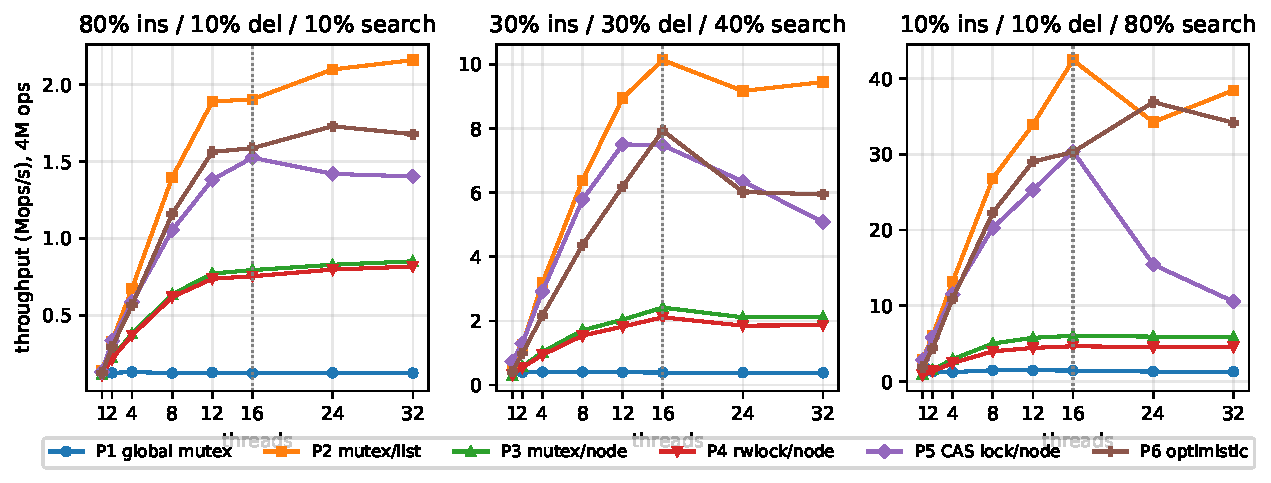
\includegraphics[width=\textwidth]{figs/q2_tput_4M.pdf}\\[1.2em]
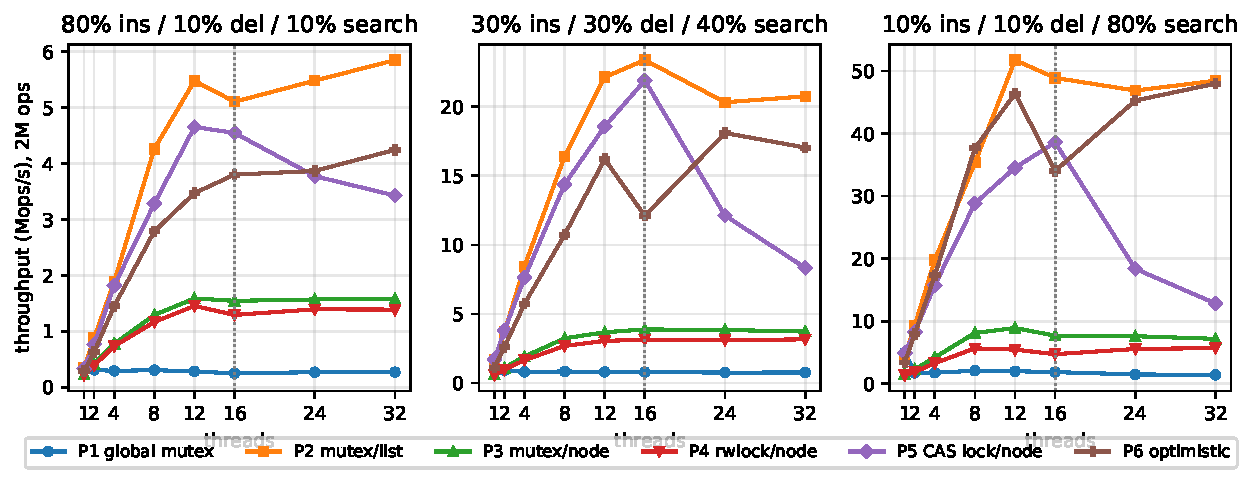
\includegraphics[width=\textwidth]{figs/q2_tput_2M.pdf}\\[1.2em]
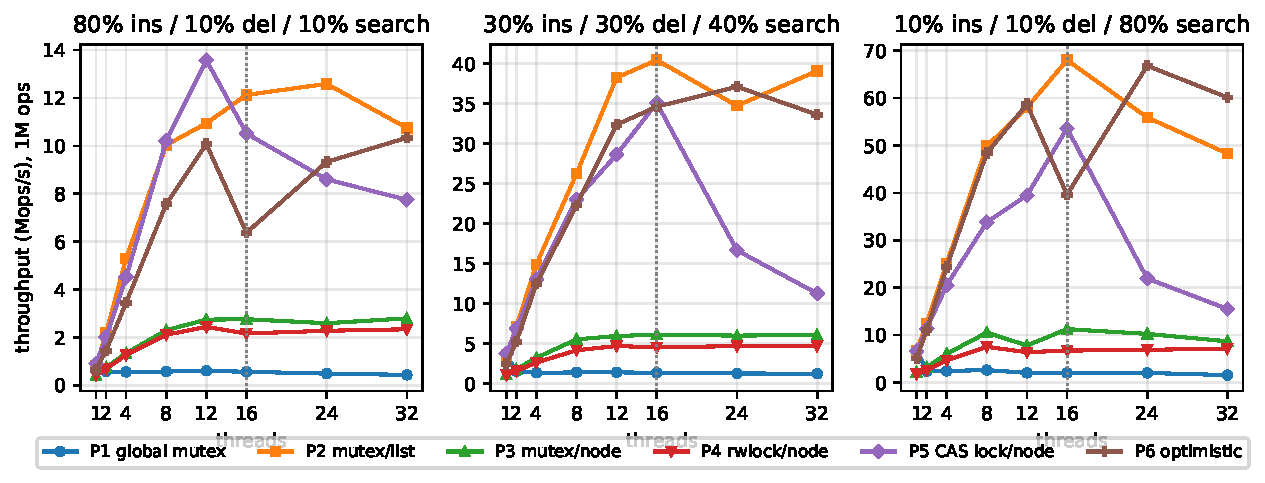
\includegraphics[width=\textwidth]{figs/q2_tput_1M.pdf}
\caption{Q2: throughput (millions of operations per second; higher is better) vs threads for 4M (top), 2M and 1M (bottom) operations.
The dotted line marks 16 hardware threads.}
\label{fig:q2}
\end{figure}

\begin{table}[h]
\centering\footnotesize
\begin{tabular}{llrrrrrrrr}
\toprule
Mix & Ops & $T{=}1$ & $T{=}2$ & $T{=}4$ & $T{=}8$ & $T{=}12$ & $T{=}16$ & $T{=}24$ & $T{=}32$ \\
\midrule
80/10/10 & 1M & P5 (0.9) & P2 (2.2) & P2 (5.3) & P5 (10.2) & P5 (13.6) & P2 (12.1) & P2 (12.6) & P2 (10.7) \\
80/10/10 & 2M & P1 (0.4) & P2 (0.9) & P2 (1.9) & P2 (4.3) & P2 (5.5) & P2 (5.1) & P2 (5.5) & P2 (5.8) \\
80/10/10 & 4M & P2 (0.1) & P5 (0.3) & P2 (0.7) & P2 (1.4) & P2 (1.9) & P2 (1.9) & P2 (2.1) & P2 (2.2) \\
\midrule
30/30/40 & 1M & P5 (3.7) & P2 (7.1) & P2 (14.9) & P2 (26.2) & P2 (38.2) & P2 (40.4) & P6 (37.1) & P2 (39.1) \\
30/30/40 & 2M & P5 (1.7) & P5 (3.8) & P2 (8.5) & P2 (16.4) & P2 (22.1) & P2 (23.4) & P2 (20.3) & P2 (20.7) \\
30/30/40 & 4M & P5 (0.7) & P5 (1.3) & P2 (3.2) & P2 (6.4) & P2 (8.9) & P2 (10.1) & P2 (9.2) & P2 (9.4) \\
\midrule
10/10/80 & 1M & P1 (6.9) & P2 (12.4) & P2 (25.1) & P2 (49.9) & P6 (58.7) & P2 (68.0) & P6 (66.8) & P6 (60.1) \\
10/10/80 & 2M & P1 (5.0) & P2 (9.3) & P2 (19.8) & P6 (37.6) & P2 (51.7) & P2 (48.9) & P2 (46.9) & P2 (48.4) \\
10/10/80 & 4M & P2 (2.9) & P2 (6.0) & P2 (13.2) & P2 (26.8) & P2 (33.9) & P2 (42.4) & P6 (36.9) & P2 (38.4) \\
\bottomrule
\end{tabular}

\caption{Q2: fastest version for every configuration, with its throughput in Mops/s. All times are in Appendix~\ref{app:q2}.}
\label{tab:q2best}
\end{table}

\paragraph{Overview.}
Figure~\ref{fig:q2} and Table~\ref{tab:q2best} show a similar picture for every mix and size. The one-mutex-per-list version (P2) was the fastest or close to it in almost all configurations.
The optimistic version (P6) and the hand-over-hand spin-lock version (P5) came next, the hand-over-hand pthread versions (P3, P4) were 2--7$\times$ slower than P2,
and the global lock (P1) did not scale. For P2 with 16 threads and 4M operations, the speed-up over the sequential run was
about 12--14$\times$ (80/10/10), 13--17$\times$ (30/30/40) and 14--15$\times$ (10/10/80). We give ranges because the sequential time varied a lot between runs:
P1, P2 and P5 run identical sequential code at $T=1$, and their nine runs for 30/30/40 with 4M operations took between 5.2 and 7.3\,s
(the lower end of each range uses the fastest of these nine runs, the upper end their median). These speed-ups are higher than the 8 physical cores. Our interpretation is that the work is dominated by
cache misses while following list pointers, and the two hardware threads of a core can overlap their misses.
Already at 2--8 threads the speed-up was slightly above the number of threads (e.g.\ 2.1--2.4$\times$ at $T=2$). We think this is at least partly because the sequential runs
were often slow: when we repeated the 30/30/40, 4M sequential run seven times, it took between 4.8 and 9.0\,s, while 2-thread runs stayed at 2.9--3.0\,s.
Our laptop was in a power-saving profile, and we suspect a single busy thread is not clocked or scheduled consistently, but we did not investigate this further.

\paragraph{P1 (one global mutex).}
P1 was slower with 2 threads than with 1 in every configuration (e.g.\ 1.4\,s $\to$ 3.0\,s for 10/10/80, 4M), and stayed flat or got slower with more threads.
This is what we expected, since only one operation can run at a time. We think the slow-down comes from the mutex and the list data moving between cores,
and from waiting threads being put to sleep and woken up by the contended mutex.

\paragraph{P2 (one mutex per list).}
With 10{,}000 lists and uniformly random $u$, two threads should rarely work on the same list at the same time, so we expect the per-list mutexes to be almost uncontended.
Each operation then costs one lock/unlock pair plus the sequential traversal, nothing is written while walking the list, and the nodes stay at 16 bytes.
P2's time dropped at least in proportion to the number of threads up to 8 threads (see the note on the sequential time above), improved a little more up to 16 (hyper-threading),
and stayed about the same at 24--32 threads.

\paragraph{P3 and P4 (pthread lock per node).}
At 16 threads and 4M operations, P3 was 2.4$\times$ (80/10/10), 4.2$\times$ (30/30/40) and 7.1$\times$ (10/10/80) slower than P2, and P4 was slower than P3. We see two likely reasons:
\begin{itemize}
\item every node visited needs a lock and an unlock, and both write to the node, so walking a list turns into a series of writes;
      nodes near the start of each list, especially the sentinel that every operation on that list locks, then have to move between cores;
\item the nodes are bigger (56 bytes with a mutex, 72 with an rwlock, vs 16), so each list covers 3.5--4.5$\times$ more cache lines.
      We could see this even at $T = 1$, where P3/P4 run the same sequential code as P1/P2 but took 2--3$\times$ longer on the 10/10/80 and 30/30/40 mixes
      (e.g.\ 4.2\,s and 4.7\,s vs 1.4\,s for 10/10/80, 4M).
\end{itemize}
The gap to P2 was smallest for the 80\% insert mix, which we think is because there the graph grows the most and all versions spend most of their time on cache misses.

We expected the read/write locks of P4 to help with the 80\% search mix, since searches can share nodes. This did not happen: P4 was 5--30\% slower than P3 in every mix.
Our understanding is that taking a read lock still writes to the lock word (to update the reader count), so it moves the cache line just like a mutex, and that glibc's rwlock is more expensive than its mutex.
Sharing would only help when readers actually wait for each other, which we expect to be rare with 10{,}000 lists.
The read-locked walk for insert/delete (Section~2.2) made P4 3--10\% faster, but it was still behind P3.

\paragraph{P5 (spin lock per node).}
P5 uses the same hand-over-hand algorithm as P3, but with a 4-byte spin lock, so its nodes are as small as P1/P2's and taking an uncontended lock is cheaper than \texttt{pthread\_mutex\_lock}.
Up to 12--16 threads it was 2--5$\times$ faster than P3 and within 10--40\% of P2, and it was even the fastest version for 80/10/10 with 1M operations at 8 and 12 threads.
Above 16 threads its throughput dropped sharply: for 10/10/80 with 4M operations, from 30 to 11\,Mops/s between $T=16$ and $T=32$.
We think this is the same effect as for P1 in Question 1. When the OS preempts a thread that holds a node lock, the threads that reach that node spin until the holder runs again,
and because every operation on a list passes through the first few nodes, one preempted holder can block several threads.

\paragraph{P6 (optimistic locking).}
P6 walks without locks, locks one or two nodes only for a short time at the end, and does not lock at all for searches. Up to 16 threads it was 20--40\% behind P2.
We think this is because it does the same traversal plus validation and occasional retries, with a slightly larger node (24 bytes, for the \texttt{deleted} flag),
while P2's locks are rarely contended in this setting anyway. Unlike P5, P6 did not slow down sharply above 16 threads; in most configurations it was about as fast at 24--32 threads as at 16.
Our explanation is that it holds its locks for such a short time that a preempted thread rarely blocks others.
For the search-heavy mix this brought it close to P2 at 24--32 threads (within about 10\%, and sometimes faster: 10/10/80, 4M, $T=24$: 0.11\,s vs 0.12\,s;
10/10/80, 1M, $T=32$: 17\,ms vs 21\,ms). For the other two mixes it stayed clearly behind P2 at 2M and 4M operations (13--59\% slower at $T=24, 32$).

\paragraph{Effect of the operation mix.}
The search-heavy mix (10/10/80) ran fastest, as the graph barely grows (+0.4M edges at 4M operations) and searches do not modify anything.
The insert-heavy mix (80/10/10) was by far the slowest, as the graph grows to more than 7$\times$ its initial size.
The mix also changed the gaps between versions: with more searches, the cost of locking every node (P3, P4) mattered more relative to the traversal, and P6's lock-free searches helped more.

\paragraph{Effect of the number of operations.}
More operations always gave lower throughput, because the lists get longer (strongly for 80/10/10, only slightly for 10/10/80). The ranking of the versions was the same for 1M, 2M and 4M operations.
Some 1M configurations finish in 15--100\,ms, so those numbers are noisier. When we repeated some 4M runs at a different time,
the results varied by up to 35\% at $T=16$ on our laptop, so we only draw conclusions from differences that are larger than this and consistent across all three sizes.

\paragraph{Summary.}
In our setup (many vertices and uniformly random operations), contention on any single list was low, and the simplest fine-grained scheme, one lock per list (P2), performed best.
Locking every node added lock operations and larger nodes without much benefit here. Among the per-node schemes, optimistic locking (P6) performed best and was the least affected by oversubscription.
We would expect the per-node schemes to do relatively better on a graph with few vertices and long, frequently accessed lists, but we did not test this.
